\documentclass{article}
\usepackage{graphicx} % Required for inserting images
\usepackage{geometry}
\usepackage[T1]{fontenc}
\usepackage[utf8]{inputenc}
\usepackage[english,russian]{babel}
\usepackage{amsmath}
\usepackage{amsthm}
\usepackage{amssymb}
\usepackage{fancyhdr}
\usepackage{setspace}
\usepackage{graphicx}
\usepackage{colortbl}
\usepackage{tikz}
\usepackage{pgf}
\usepackage{subcaption}
\usepackage{caption}
\usepackage{listings}
\usepackage{indentfirst}
\usepackage[
backend=biber,
style=numeric,
maxbibnames=99
]{biblatex}
\addbibresource{refs.bib}
\usepackage[colorlinks,citecolor=blue,linkcolor=blue,bookmarks=false,hypertexnames=true, urlcolor=blue]{hyperref} 
\usepackage{indentfirst}
\usepackage{mathtools}
\usepackage{booktabs}
\usepackage[flushleft]{threeparttable}
\usepackage{tablefootnote}

\usepackage{chngcntr} % нумерация графиков и таблиц по секциям
\counterwithin{table}{section}
\counterwithin{figure}{section}


\title{Software Requirements Specification -- социальная сеть "Мастера судоку"}
\author{ Роман Сахаров}
\date{}

\begin{document}

\maketitle

\section*{Введение}
\subsection*{Цель проекта}
Создать мобильное приложение, реализующее функционал социальной сети по тематике судоку и совмещенное непосредственно с игрой. Приложение создаётся, чтобы предоставить пользователям необычную и интересную возможность времяпрепровождения в виде совмещённой игры-головоломки и социальной сети. 

\subsection*{Целевая аудитория}
\begin{itemize}
    \item Фанаты игры судоку, которые хотят пообщаться по этой теме 
    \item Люди, которые ищут, чем заняться во время поездки или ожидания в очереди
    \item Игроки, желающие помериться силами и умением решать судоку
    \item  Начинающие игроки, которые получат возможность пообщаться с профи и перенять их
опыт
    \item Люди, которые хотят "держать мозг в тонусе"\, решая головоломки в интересном формате
\end{itemize}

\subsection*{Голоссарий}
\begin{enumerate}
    \item  \textbf{Головоломка} - непростая задача, для решения которой, как правило, ребуется сообразительность, а не специальные знания высокого уровня.
    \item \textbf{Приложение} - подразумевается мобильное приложение, т.е. программное 
    обеспечение, которое устанавливается на мобильных устройствах, таких как смартфоны или планшеты.
    \item \textbf{Тематическая социальная сеть} - онлайн-платформа, которая используется для общения, знакомств, создания социальных отношений между людьми, которые имеют схожие интересы
    \item \textbf{Валидное судоку (Valid Sudoku)} - разработанное мной на 2-м курсе мобильное приложение для игры в судоку, включающее функционал генерации судоку разных размеров и уровней сложности, сбор статистики и возможность сменить оформление приложения

\end{enumerate}

\section*{Обзор системы}

\subsection*{Описание продукта}
Итоговый продукт должен представлять из себя мобильное приложение + сервер. 

Сервер должен заниматься обработкой данных и вычислениями, а также реализовывать логику социальной сети, предоставляя наружу API-интерфейс. 

Мобильное приложение будет "продолжением", развитием приложения "Валидное судоку" (т.е. должно предоставлять все те же возможности, дополняя их новым функционалом). Таким образом, в добавок к возможности играть в судоку, в приложении появится интерфейс социальной сети с чатами и страничками пользователей, а также возможность участвовать в соревновательных режимах.

\subsection*{Дизайн и реализация}

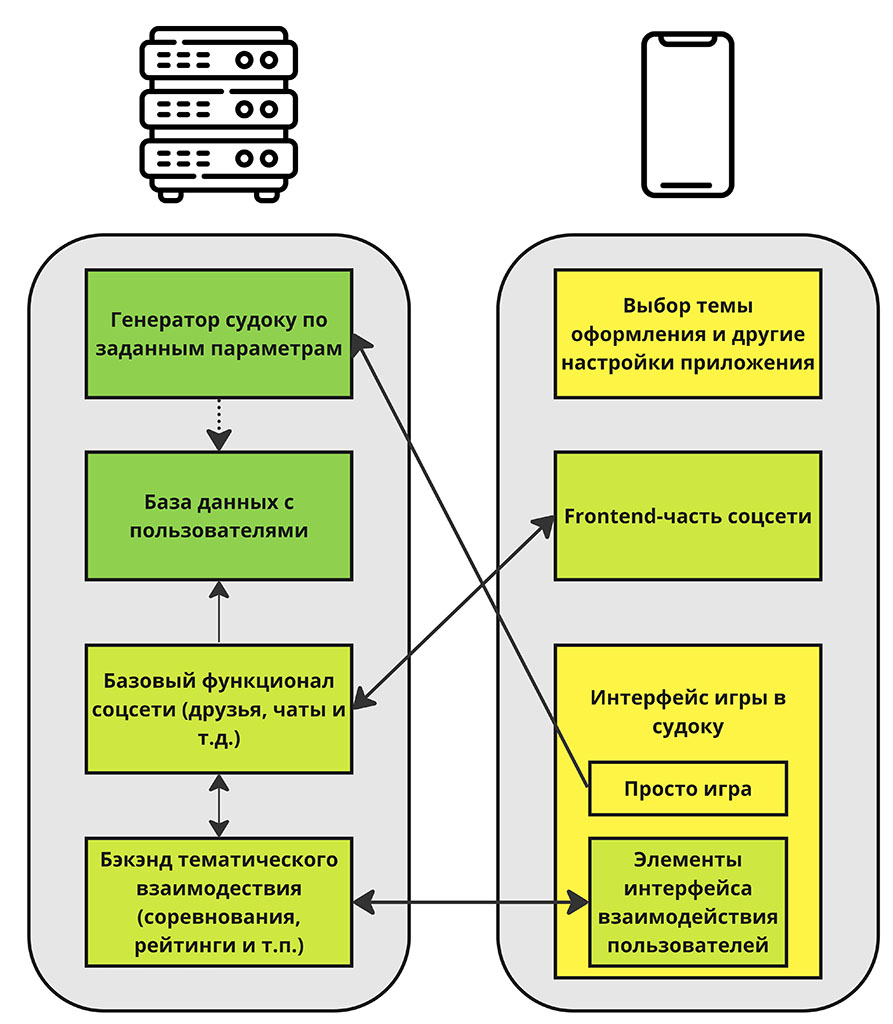
\includegraphics[scale=0.3]{scheme.jpg}

Основным инструментом для разработки frontend-части (т.е. мобильного приложения) остаётся Flutter. Он кроссплатформенный, довольно удобный для разработки, а проблемы с производительностью будут решены через вынесение на сервер больших вычислительных процессов (генерация, анализ статистики).

Как раз все эти вычислительные алгоритмы планируется писать на C++ (с распараллеливанием для ускорения).
Backend сервера с логикой соцсети будет реализован на Flask (Python).

Для хранения данных будет использоваться БД SQLite (работа с БД будет производиться через ORM SQLAlchemy-flask)

\subsection*{Рабочая среда}

Серверная часть приложения будет развернута на удалённом сервере под управлением ОС Ubuntu-22.04.

Мобильное приложение сможет работать на мобильных устройствах под управлением Android и IOS (Flutter поддерживает также работу под Windows, однако корректность работы программы с данной ОС не гарантируется)

\subsection*{Классы и характеристики пользователей}
\begin{itemize}
    \item \textbf{Зарегистрированный пользователь}, который имеет учётную запись в социальной сети, может общаться с другими пользователями, добавляться в друзья и участвовать в multiplayer-активностях
    \item \textbf{Незарегистрированный пользователь}. Пользуется приложением, как обычной игрой, по сути копирующим функционал текущей версии "Валидного судоку" (за исключением генерации судоку и обработки статистики на сервере)
\end{itemize}

\subsection*{Документация пользователя}
Пользователям при работе с приложением (для игры и общения) не будет нужна документация. Однако для взаимодействия между сервером и клиентом потребуется задокументированный API

\subsection*{Функциональные требования}

Готовый продукты должен уметь следующее:

\begin{itemize}
    \item Предоставлять пользователям базовую возможность игры в судоку
    \item Предоставлять возможность общения в чатах (личных и групповых)
    \item Устанавливать связи между пользователями (друзья)
    \item Собирать статистику по пользователям и их играм и формировать на их основе игровые рейтинги
    \item Предоставлять возможность играть в multiplayer режимы
\end{itemize}

\subsection*{Нефункциональные требования}

Готовый продукты должен удовлетворять следующим условиям:

\begin{itemize}
    \item Кроссплатформенность (для Android и IOS)
    \item Монетизация за счёт рекламы
    \item Кастомизируемость интерфейса приложения (посредством тем оформления)
\end{itemize}

\subsection*{Тестирование}

\begin{itemize}
    \item \textbf{Модульное тестирование сервера}. Все компоненты сервера (алгоритмы генерации, работа с БД и т.д.) должны быть протестированы по-отдельности.
    \item \textbf{Интеграционное тестирование}. Должно быть протестировано взаимодействие клиента и сервера.
    \item \textbf{QA тестирование}. Продукт должен быть протестирован пользователями (тестировщиками), которые будут использовать приложение в приближенных к реальным сценариях.
\end{itemize}

\section*{Задачи проекта}

\begin{enumerate}
    \item Вынести процесс генерации судоку на сервер
    \item Спроектировать будущее веб-приложение
    \item Организовать  базу данных на сервере
    \item Реализовать базовое взаимодействие между пользователями (общение, добавление в друзья)
    \item Добавить элементы соревновательности (напр. рейтинг)
    \item Добавить различные тематические элементы во взаимодействие между пользователями
    \item Внедрить в приложение "Валидное судоку"\ функционал клиентской части
    \item Протестировать готовый продукт
    \item Развернуть сервер и обновить мобильное приложение
\end{enumerate}


\end{document}
